\documentclass[../main.tex]{subfiles}

\begin{document}

\subsection{Django}

Se utiliza Django para proporcionar un API REST que da acceso a las imágenes del dataset. Así como proporcionar un listado de las url de las imágenes organizadas por letras. Este listado será usado por la aplicación de entrenamiento para extraer las características de las imágenes.

Para la ejecución del proyecto se utiliza Pycharm~\cite{pycharm}, que se encarga de la compilación y ejecución en un servidor web local. También se utiliza Django REST Framework \cite{restframework} para facilitar la creación de un endpoint. Se proporciona el código completo del proyecto, así que se detallan solamente los aspectos más importantes:

\begin{itemize}
    \item Ejecución en un entorno local: Se utiliza el IDE Pycharm para ejecutar el proyecto, para ello se establece la siguiente configuración~\ref{figure2}
    
    \item Settings.py: Configuración de la ruta donde se encuentran las imágenes del dataset. 
    \begin{lstlisting}[style=stylepython]
    STATIC_URL = '/static/'
    DEFAULT_SCHEME = "http://192.168.1.5:8000"
    
    MEDIA = 'media'
    DATASET = 'dataset'
    
    MEDIA_URL = '/media/'
    MEDIA_ROOT = os.path.join(BASE_DIR, "media")
    
    MEDIA_DEFAULT = DEFAULT_SCHEME + MEDIA_URL
    DATASET_ROOT_DIR = os.path.join(MEDIA_ROOT, 'dataset')
    
    DATASET_URL = DEFAULT_SCHEME + MEDIA_URL + DATASET + "/"
\end{lstlisting}
    \item Estructura de la carpeta media: Contiene el conjunto de datasets utilizados en el proyecto, están numerados del 1 al 6 y dentro de cada uno se organizan por letras~\ref{figure3}.
     \item Obtener un listado de las imágenes: Proporcionar un endpoint para obtener en formato JSON un listado de todas las imágenes organizadas por letras.
     \begin{lstlisting}[style=stylepython]
     class ImagesListAPI(APIView):
    """ List of urls images by letters"""
    def get(self, request):
        labelsClass = ["A", "B", "C", "D", "E", "F", "G", "H", "I", "K",
                       "L", "M", "N", "O", "P", "Q", "R", "S", "T", "U",
                       "V", "W", "X", "Y"]
        json_data = {}
        train_folder = os.path.join(settings.DATASET_ROOT_DIR, 'train')
        for letter in labelsClass:
            list_images = []
            for i in range(1, 7):
                folder_data = os.path.join(train_folder, str(i), letter)
                images_list = os.listdir(folder_data)
                for imageName in images_list:
                    url = settings.DATASET_URL + "train" + "/" + str(i) + "/" + letter + "/" + imageName
                    list_images.append(url)
            json_data[letter] = list_images
        return JsonResponse(json_data)
     \end{lstlisting}
\end{itemize}

\begin{figure}[h]
\centering 
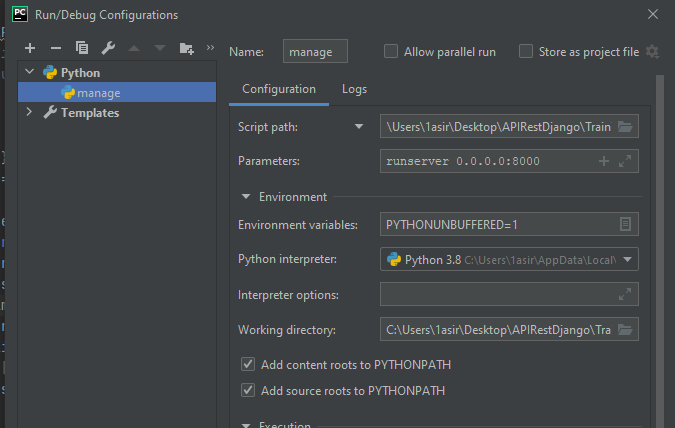
\includegraphics[width=1\textwidth]{images/apirest/api1.PNG}
\caption{Configuración de ejecución en Pycharm}
\label{figure2}
\end{figure}

\begin{figure}[h]
\centering 
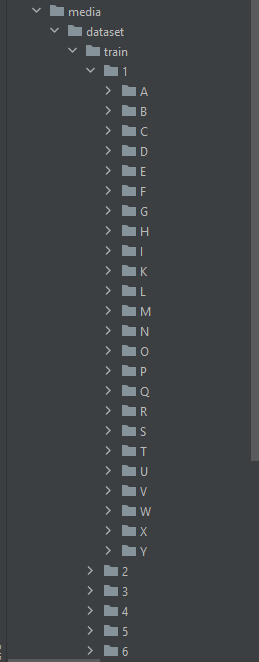
\includegraphics[width=0.5\textwidth]{images/apirest/api7.PNG}
\caption{Organización de la carpeta media}
\label{figure3}
\end{figure}

\newpage

El resultado de este componente del sistema se muestra en la figura  \ref{figure4} y será usado por la app de entrenamiento para obtener las imágenes a analizar. Tener este componente organizado por diferentes dataset numerados nos permite realizar pruebas realizando entrenamientos sobre sólo una selección de ellos y realizar modificaciones sobre cuáles de los dataset se van a incluir en el entrenamiento del sistema.
\begin{figure}[h]
\centering 
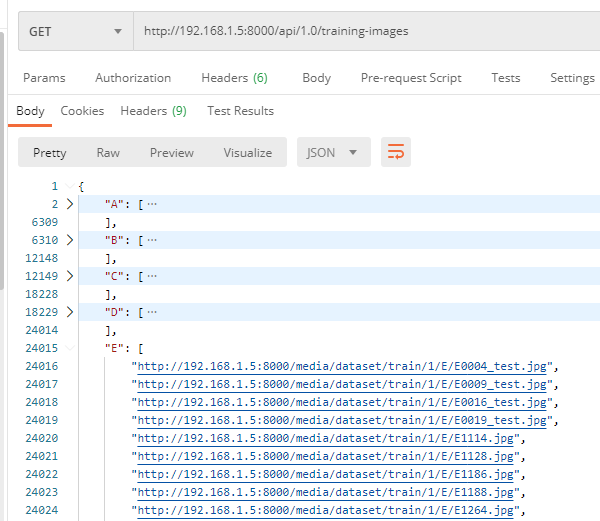
\includegraphics[width=1\textwidth]{images/apirest/api6.PNG}
\caption{Listado en formato JSON de las imágenes a analizar organizadas por letras.}
\label{figure4}
\end{figure}




\end{document}